% Chapter Template

\chapter{Introduction} % Main chapter title

\label{Chapter 1} % Change X to a consecutive number; for referencing this chapter elsewhere, use \ref{ChapterX}

\lhead{Chapter 1. \emph{Introduction}} % Change X to a consecutive number; this is for the header on each page - perhaps a shortened title

%----------------------------------------------------------------------------------------
%	SECTION 1
%---------------------------------------------------------------------------------------
\section{Clustering}
Clustering analysis  has been an  emerging  research  issue in data mining due its variety of  applications.Clustering is the task of dividing data points into a number of groups such that data points in the same groups are more similar to other data points in the same group than those in other groups. In simple words, the aim is to segregate groups with similar traits and assign them into clusters. 

Clustering is  used in many fields like Market research,Biology,Search result grouping,Analysis of antimicrobial activity,Human genetic clustering etc.We are trying to use clustering to group similar motion segments in dance videos.In particular,we have clustered the \textbf{BharataNatyam} natta videos.


With the advent of many data clustering  algorithms  in  the  recent  few  years  and its extensive  use in  wide variety of applications,  including image processing, computational biology, mobile communication, medicine and economics,  has  lead  to  the  popularity of  this  algorithms.Main  problem with  the data clustering algorithms is   that it  cannot  be  standardized.   Algorithm developed may  give  best  result  with one type of data set  but  may  fail or  give  poor  result with  data set of other types.  Although  there  has  been  many  attempts   for  standardizing  the  algorithms  which can   perform   well   in  all  case  of scenarios but  till  now  no major accomplishment  has been achieved.

Many clustering algorithms  have  been  proposed so far. However, each  algorithm has its own  merits and demerits  and cannot  work  for  all  real  situations.So,we have looked into different clustering algorithms and found that \textbf{Spectral Clustering}  suits our purpose well.We have explained spectral clustering in the coming chapters.

\section{Motion Representation \& Similarity Measure}

The problem of clustering in the domain of dance is difficult compared to other domains because there was no fixed representation for the dance motions.we have used \textbf{optical flow} to represent each motion as a feature vector.Since each motion spans different no of frames,the size of feature vector is different for different motions.

In clustering,for deciding whether two motions should go to same cluster or different clusters,we should have a measure to compare two motions.Each motion spans across different no of frames even the similar ones(for example motion1 may span 10 frames while motion2 may frame 15 frames).Depending on the frame rate,even the similar motions may have different frames.Hence we need to design a similarity measure to compare different sized feature vectors corresponding to each motion.

The similarity measure should be more for similar motions and less for different motions and it should be able to compare motions with different no of frames.In this report,we proposed a measure which deals with all these problems and giving a good accuracy.






\section{Problem Statement}

The goal of this research is to effectively represent motions and design a similarity measure to cluster the motions of the given \textbf{BharataNatyam} dance videos.Specifically we have tested our approach on bharatanatyam second Adavu \textbf{Natta}.The input given was a set of videos where a dancer will be performing a Natta and a motion annotation file representing the motion frame details in the video.

\section{DataSet}

The domain we are dealing is Indian Bharatanatyam. Adavu’s are the ba-
sic units of Bharatanatyam. While performing Adavu’s, the dancer stamps,
rubs, touches, slides on the ground in different ways in synchronization with the music.There are 15 Adavus in which \textbf{Natta} is the second one which we are dealing.In Natta,there are again 8 variations.

For each variation, there are 9 sets of data corresponding to 9 dancers, each set has a video and an RGB image, a skeleton image, a depth image and a mat file containing information of skeleton image for each frame in the video as shown in the fig 3.

\begin{figure} [!htbp]
\centering    
\subfigure[RGB Image]{\label{RGB Image}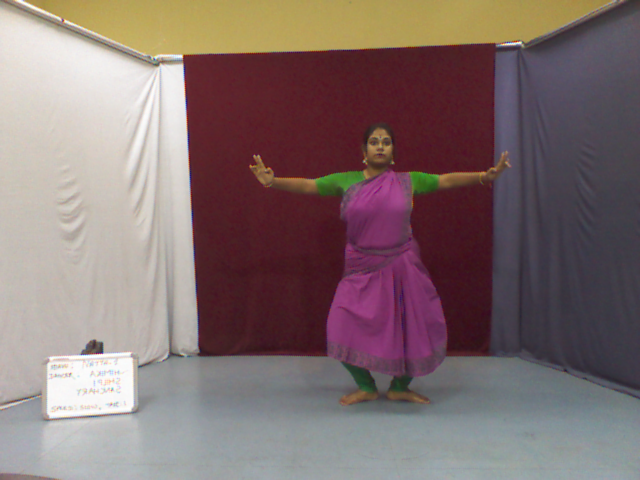
\includegraphics[width=42mm]{rgb.png}}
\subfigure[Depth Image]{\label{Depth Image}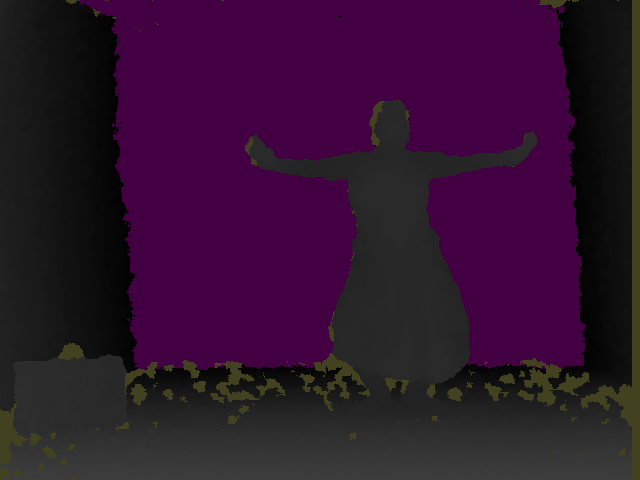
\includegraphics[width=42mm]{depth.png}}
\subfigure[Skeleton Image]{\label{Skeleton Image}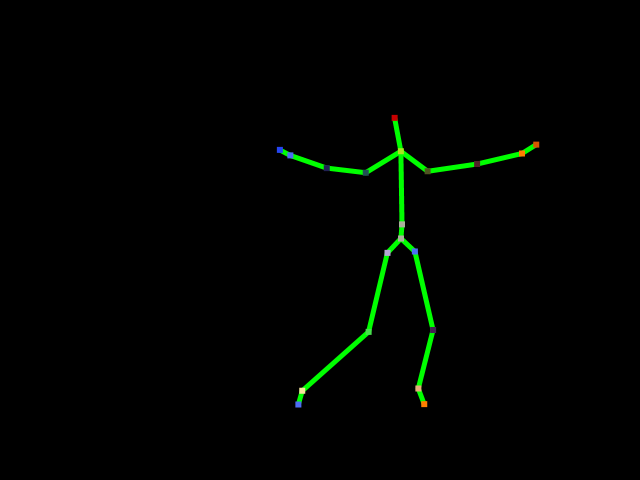
\includegraphics[width=42mm]{skeleton.png}}
\caption{Different Channels for each frame in video}
\end{figure}


In this semester,we have worked on clustering of motions using RGB image dataset.The following picture shows the scale of the data we worked on.



\begin{figure} [!htbp]
\centering
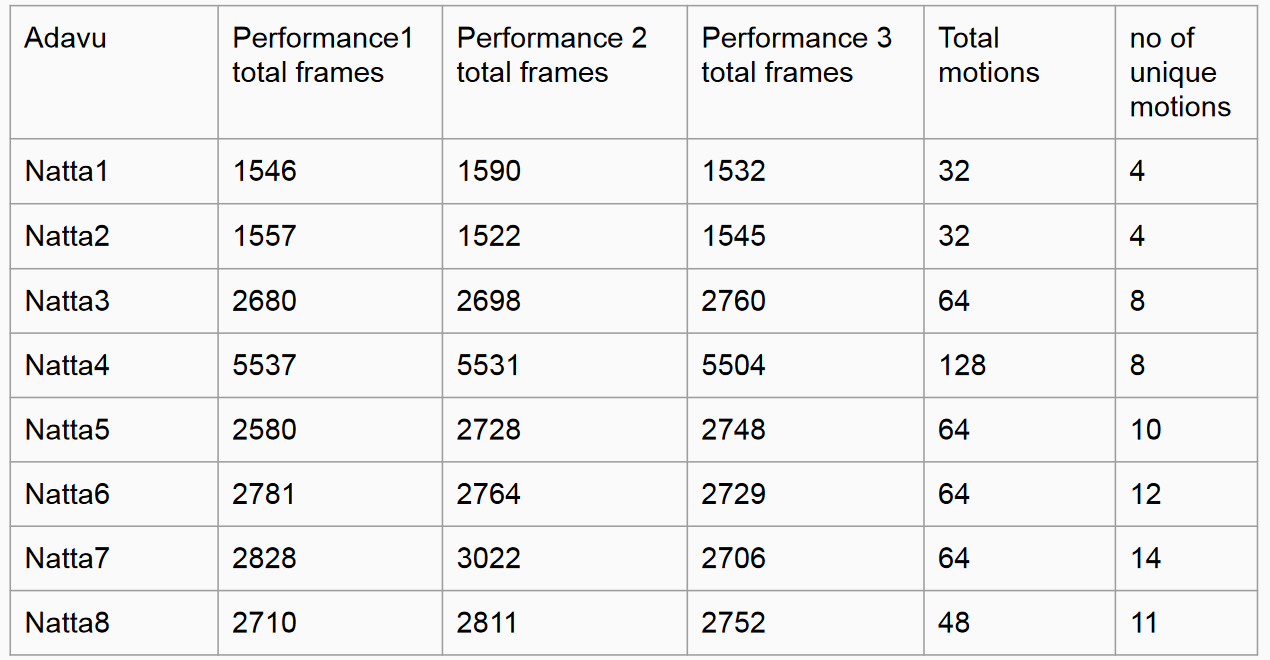
\includegraphics[width=120mm]{Pictures/data.png}
\caption{Picture showing our DataSet}
\end{figure}


Along with these videos,we also have a motion annotation file with each video consisting of motion start and end frame details for each motion in the video.  

\section{Organization of this Report}

Chapter 2 introduces the various techniques used in our approach.we explained the optical flow which we used it to represent motions in our scenario.we also explained the Dynamic Time Warping which is used as the similarity measure and then the Spectral Clustering.

In Chapter 3,we have outlined the approach we followed and the results we obtained on the mentioned dataset and discussed some insights on the results.Finally ,the conclusions will be summarized and the evaluation measure will described.Also possible areas for future work are stated briefly.